\documentclass[class=article, crop=false]{standalone}
\usepackage{tikz}
\usepackage{subcaption}
\usetikzlibrary{calc}

\begin{document}
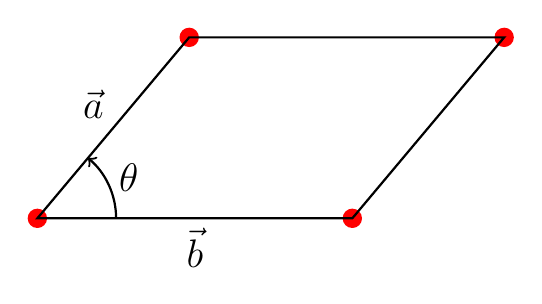
\begin{tikzpicture}
    % Define the lengths of the sides and the angle
    \def\a{4}  % length of side a
    \def\b{3}  % length of side b
    \def\angle{50}  % angle between sides a and b

    % Calculate the coordinates of the points
    \coordinate (A) at (0, 0);
    \coordinate (B) at (\a, 0);
    \coordinate (C) at ({\a + \b*cos(\angle)}, {\b * sin(\angle)});
    \coordinate (D) at ({\b * cos(\angle)}, {\b * sin(\angle)});

    
    % Creates nodes at vertices
    \fill[red]  (A) circle(3.5pt) (B) circle(3.5pt) (C) circle(3.5pt) (D) circle(3.5pt);

    % Draw the oblique unit cell
    \draw[thick] (A) -- (B) -- (C) -- (D) -- cycle;

    %Draw lattice parameters
    \node[anchor={-\angle}] at ($(A)!0.5!(D)$) {\Large $\vec{a}$};
    \node[below] at ($(A)!0.5!(B)$) {\Large $\vec{b}$};
    
    % Optional: add angle markers
    \draw[thick, ->] (A) ++(1,0) arc[start angle=0, end angle=\angle, radius=1] node[midway, anchor={150+\angle}] {\Large $\theta$};
\end{tikzpicture}
\end{document}